\documentclass{article}

\usepackage{graphicx}
\usepackage{tikz}
\usepackage{tikzsymbols}
\usetikzlibrary{calc,patterns,shapes.geometric}
\pagestyle{empty}
\usepackage[margin=0pt]{geometry}
\geometry{papersize={14in,12in}}

\def\centerarc[#1](#2)(#3:#4:#5){\draw[#1] ($(#2)+({#5*cos(#3)},{#5*sin(#3)})$) arc (#3:#4:#5);}

\begin{document}
	\begin{figure}
		\centering
		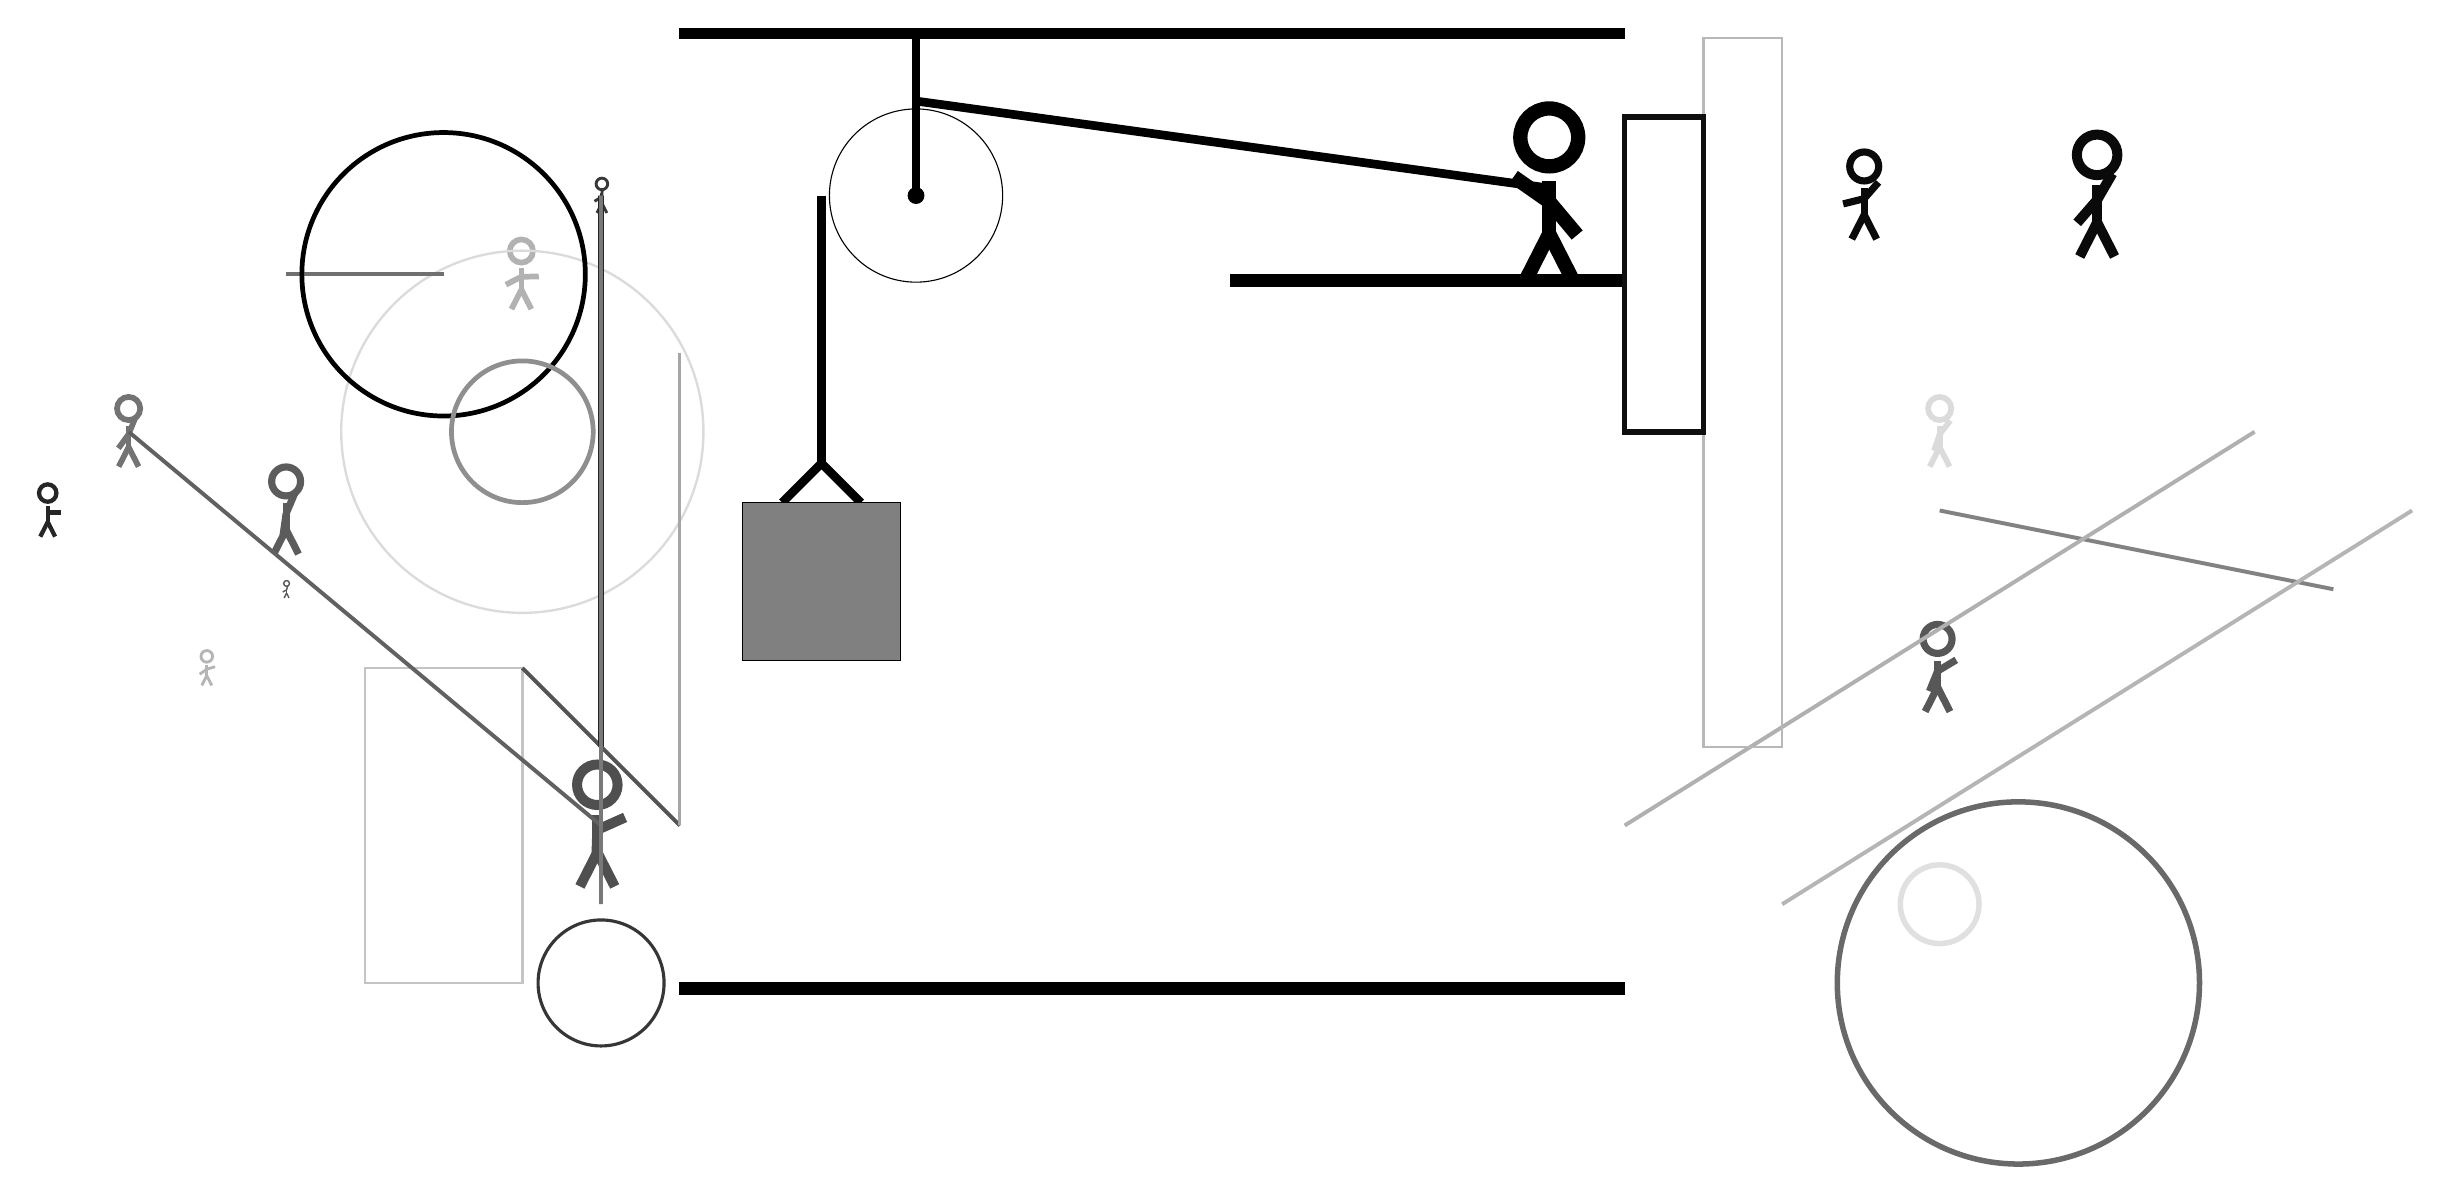
\begin{tikzpicture}
			%%%%% START %%%%%
			
			\draw[fill=black] (-2, 9) rectangle (10, 9.125);
			
			\draw (1, 7) circle (1.1);
			\draw[fill=black] (1, 7) circle (0.1);
			\draw[line width=1.1mm] (1, 9) -- (1, 7);
			
			\draw[line width=1.1mm](-0.7, 3.1) --  (-0.2, 3.6) -- (0.3, 3.1);
			\draw[fill=black!50] (-1.2, 3.1) rectangle (0.8, 1.1);
			
			\draw[line width=1.1mm](-0.2, 7) -- (-0.2, 3.6);
			\centerarc[line width=1.1mm](1, 7)(90:180:1.2000000000000002)
			\draw[line width=1.1mm](1, 8.2) -- (9, 7.1);
			
			\node at (9, 7) {\Strichmaxerl[10][-35][-50]};
			\draw[fill=black] (5, 6) rectangle (10, 5.85);
			
			\node[line width=0.5mm, color=black!96] at (13, 7) {\Strichmaxerl[5][14][49]};
			
			\draw[line width=0.2mm, color=black!89] (-3, -1) rectangle (-3, 1);
			\node[line width=0.3mm, color=black!30] at (-4, 6) {\Strichmaxerl[4][27][1]};
			\node[line width=0.2mm, color=black!55] at (-9, 4) {\Strichmaxerl[4][54][68]};
			\node[line width=0.5mm, color=black!66] at (14, 1) {\Strichmaxerl[5][68][31]};
			
			\draw [line width=0.5mm, color=black!19](13, -2) circle (0.0);
			\draw[line width=0.5mm, color=black!49](14, 3) -- (19, 2);
			
			\draw [line width=0.4mm, color=black!79](-3, -3) circle (0.8);
			\node[line width=0.6mm, color=black!96] at (16, 7) {\Strichmaxerl[7][49][60]};
			
			\draw[line width=0.3mm, color=black!23] (-4, -3) rectangle (-6, 1);
			\node[line width=0.5mm, color=black!69] at (-3, -1) {\Strichmaxerl[7][88][24]};
			\draw[line width=0.5mm, color=black!67](-4, 1) -- (-2, -1);
			\node[line width=0.4mm, color=black!29] at (-8, 1) {\Strichmaxerl[2][35][17]};
			
			\node[line width=0.6mm, color=black!65] at (-7, 2) {\Strichmaxerl[1][29][74]};
			\draw[line width=0.5mm, color=black!29](12, -2) -- (20, 3);
			\draw[line width=0.5mm, color=black!31](10, -1) -- (18, 4);
			
			\node[line width=0.7mm, color=black!14] at (14, 4) {\Strichmaxerl[4][71][52]};
			\draw[line width=0.3mm, color=black!28] (12, 9) rectangle (11, 0);
			\draw [line width=0.7mm, color=black!59](15, -3) circle (2.3);
			\node[line width=0.3mm, color=black!78] at (-3, 7) {\Strichmaxerl[2][31][88]};
			\draw [line width=0.3mm, color=black!14](-4, 4) circle (2.3);
			\draw[line width=0.5mm, color=black!56](-5, 6) -- (-7, 6);
			\draw [line width=0.6mm, color=black!100](-5, 6) circle (1.8);
			\node[line width=0.3mm, color=black!64] at (-7, 3) {\Strichmaxerl[5][82][67]};
			\draw [line width=0.6mm, color=black!44](-4, 4) circle (0.9);
			\draw [line width=0.7mm, color=black!12](14, -2) circle (0.5);
			\node[line width=0.4mm, color=black!85] at (-10, 3) {\Strichmaxerl[3][90][0]};
			\draw[line width=0.4mm, color=black!35] (-2, 5) rectangle (-2, -1);
			\draw[line width=0.7mm, color=black!85] (-3, 0) rectangle (-3, 7);
			\draw[line width=0.5mm, color=black!62](-3, -1) -- (-9, 4);
			\draw[line width=0.5mm, color=black!53] (-3, -2) rectangle (-3, 7);
			
			\draw[line width=0.7mm, color=black!94] (10, 8) rectangle (11, 4);
			
			\draw[fill=black] (-2, -3) rectangle (10, -3.15);
			
			%%%%% END %%%%%
		\end{tikzpicture}
	\end{figure}	
\end{document}